
\begin{question}
Let's continue conducting a Box-Jenkins procedure for the differenced log(gas) time series.

You can load the gas dataset in R by importing forecast library or if you use other programming languages you can download it \href{https://github.com/vincentarelbundock/Rdatasets/blob/master/csv/forecast/gas.csv}{here}.

\begin{figure}[H]
\centering
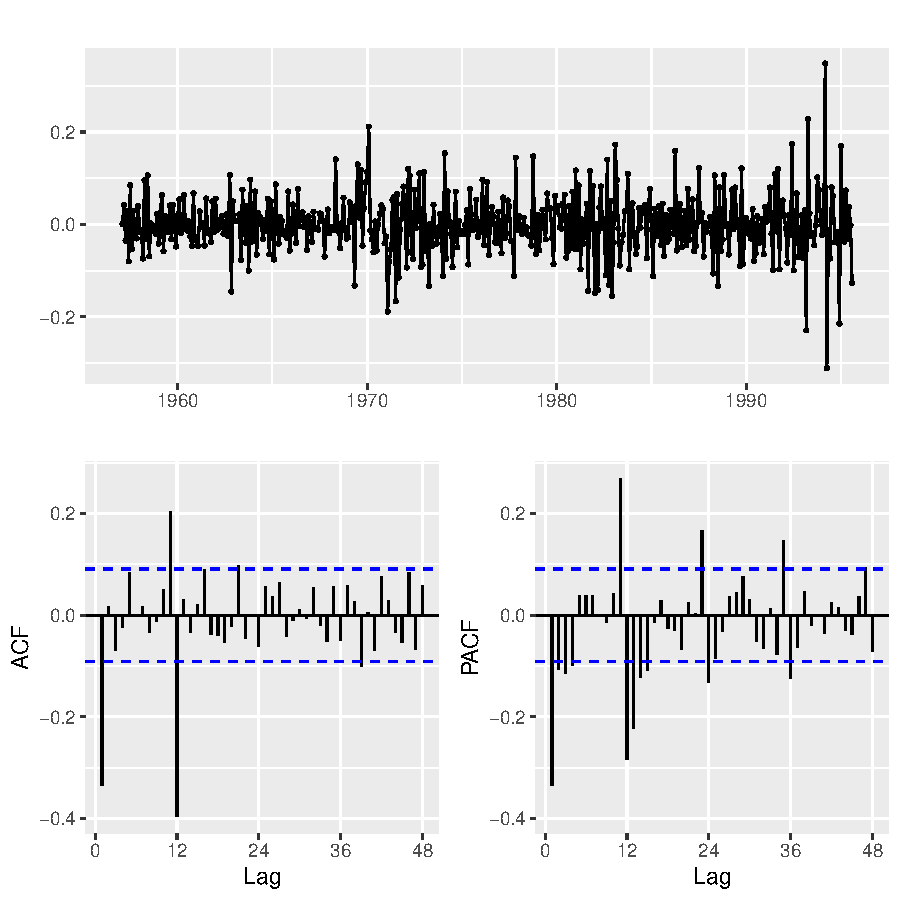
\includegraphics{unnamed-chunk-1-1-5.pdf}
\caption{plot of chunk unnamed-chunk-1}
\end{figure}

Now let's determine the parameters for SARIMA model.

By analysing ACF and PACF functions answer, what can the underlying SARMA(p,q) process for the transformed and differenced gas series be?
\begin{answerlist}
  \item SARMA(1,0){[}1,0{]}
  \item SARMA(0,1){[}0,0{]}
  \item SARMA(0,1){[}0,1{]}
  \item SARMA(0,0){[}1,0{]}
  \item SARMA(0,0){[}0,1{]}
  \item SARMA(1,0){[}0,0{]}
\end{answerlist}
\end{question}

\begin{solution}
MA process shows a gradually declining PACF and the ACF has a 1st significant lag corresponding to MA part and 12th significant lag corresponding to seasonal MA part.
\end{solution}

